%% abtex2-modelo-projeto-pesquisa.tex, v-1.9.7 laurocesar
%% Copyright 2012-2018 by abnTeX2 group at http://www.abntex.net.br/ 
%%
%% This work may be distributed and/or modified under the
%% conditions of the LaTeX Project Public License, either version 1.3
%% of this license or (at your option) any later version.
%% The latest version of this license is in
%%   http://www.latex-project.org/lppl.txt
%% and version 1.3 or later is part of all distributions of LaTeX
%% version 2005/12/01 or later.

\documentclass[
	% -- opções da classe memoir -https://www.folha.uol.com.br/-
	12pt,				% tamanho da fonte
	% openright,			% capítulos começam em pág ímpar (insere página vazia caso preciso)
	oneside,			% para impressão apenas em frente, nao frente verso. Oposto a twoside
	a4paper,			% tamanho do papel. 
	sumario=tradicional,
	% -- opções da classe abntex2 --
% 	chapter=TITLE,		% títulos de capítulos convertidos em letras maiúsculas
	%section=TITLE,		% títulos de seções convertidos em letras maiúsculas
	%subsection=TITLE,	% títulos de subseções convertidos em letras maiúsculas
	%subsubsection=TITLE,% títulos de subsubseções convertidos em letras maiúsculas
	% -- opções do pacote babel --
	english,			% idioma adicional para hifenização
	french,				% idioma adicional para hifenização
	spanish,			% idioma adicional para hifenização
	brazil,				% o último idioma é o principal do documento
]{abntex2}

% ---
% PACOTES
% ---

% ---
% Pacotes fundamentais 
% ---
% \usepackage{helvet}
% \renewcommand{\familydefault}{\sfdefault}
% \usepackage{times}
\usepackage{lmodern}			    % Usa a fonte Latin Modern
\usepackage[T1]{fontenc}		% Selecao de codigos de fonte.
\usepackage[utf8]{inputenc}		% Codificacao do documento (conversão automática dos acentos)
\usepackage{indentfirst}		% Indenta o primeiro parágrafo de cada seção.
\usepackage{color}				% Controle das cores
\usepackage{graphicx}			% Inclusão de gráficos
\usepackage{microtype} 			% para melhorias de justificação
\usepackage{lipsum}				% para geração de dummy text
% ---
\usepackage{todonotes}

\usepackage{float}
\usepackage{amssymb}
\usepackage{amsmath}
% ---
% Pacotes de citações
% ---
% \usepackage[brazilian,hyperpageref]{backref}	 % Paginas com as citações na bibl
\usepackage[alf]{abntex2cite}	% Citações padrão ABNT
\usepackage{subcaption}

\DeclareMathOperator*{\argmin}{argmin}

% --- 
% % CONFIGURAÇÕES DE PACOTES
% % --- 

% ---
% Informações de dados para CAPA e FOLHA DE ROSTO
% ---
\titulo{Reconstrução de curvas por meio de características robustas extraídas de imagens}
\autor{%
  UNIVERSIDADE DE SÃO PAULO
  \par
  Instituto de Ciências Matemáticas e de Computação}
\local{Brasil}
\data{2020}
\instituicao{%
  \textbf{Graduando:} André Luís Mendes Fakhoury
  \par
  \textbf{Orientador:} João do Espirito Santo Batista Neto}
\tipotrabalho{Iniciação Científica}
\preambulo{Projeto de Pesquisa apresentado à FAPESP para solicitação de Bolsa de Pesquisa de Iniciação Científica (IC).}
% ---

% ---
% Configurações de aparência do PDF final

% alterando o aspecto da cor azul
\definecolor{blue}{RGB}{41,5,195}
\definecolor{black}{RGB}{0,0,0}

% informações do PDF
\makeatletter
\hypersetup{
     	%pagebackref=true,
		pdftitle={\@title}, 
		pdfauthor={André Luís Mendes Fakhoury},
    	pdfsubject={\imprimirpreambulo},
	    pdfcreator={LaTeX with abnTeX2},
		pdfkeywords={abnt}{latex}{abntex}{abntex2}{projeto de pesquisa}, 
		colorlinks=true,       		% false: boxed links; true: colored links
    	linkcolor=black,          	% color of internal links
    	citecolor=black,        		% color of links to bibliography
    	filecolor=magenta,      		% color of file links
		urlcolor=black,
		bookmarksdepth=4
}
\makeatother
% --- 

% --- 
% Espaçamentos entre linhas e parágrafos 
% --- 

% O tamanho do parágrafo é dado por:
\setlength{\parindent}{1.3cm}

% Controle do espaçamento entre um parágrafo e outro:
\setlength{\parskip}{0.2cm}  % tente também \onelineskip
\setlength{\marginparwidth}{2cm}

% \DoubleSpacing

% ---
% compila o indice
% ---
\makeindex
% ---

% ----
% Início do documento
% ----

\begin{document}

% Seleciona o idioma do documento (conforme pacotes do babel)
%\selectlanguage{english}
\selectlanguage{brazil}

% Retira espaço extra obsoleto entre as frases.
\frenchspacing 

% ----------------------------------------------------------
% ELEMENTOS PRÉ-TEXTUAIS
% ----------------------------------------------------------
% \pretextual

% ---
% Folha de rosto
% ---
 \imprimirfolhaderosto
% ---

% ---
% Resumo
% ---
\begin{resumoumacoluna}

Um dos desafios atuais da área de processamento de imagens e visão computacional é o mapeamento de características robustas entre espaços bidimensionais e tridimensionais. A simplificação deste processo pode ser feita através da redução da quantidade de informações, como, por exemplo, representar curvas a partir de pontos (denominados características robustas ou pontos importantes), de forma que estas possam ser reconstruídas através destes com um erro mínimo. Assim, contornos de imagens podem ser extraídos e analisados como curvas discretas e, com isso, reduzidos a finitos pontos importantes. Portanto, a pesquisa analisará a extração de pontos importantes de curvas discretas e a seguinte reconstrução de curvas a partir destes, por meio de curvas poligonais. Este estudo insere-se em umas das linhas de atuação do projeto temático \textit{FAPESP 2019/07316-0}, que visa a reconstrução de faces humanas a partir de informações reduzidas do domínio.
 
 \vspace{\onelineskip}
 
 \noindent
 \textbf{Palavras-chave}: imagens. curvas. características robustas. restauração.
\end{resumoumacoluna}

% ---
% inserir o sumario
% ---
\pdfbookmark[0]{\contentsname}{toc}
\tableofcontents*
\cleardoublepage
% ---

% ----------------------------------------------------------
% ELEMENTOS TEXTUAIS
% ----------------------------------------------------------
\textual
\pagestyle{simple}

\begingroup
\let\clearpage\relax

% ----------------------------------------------------------
% Introdução
% ----------------------------------------------------------
\chapter{Introdução e justificativa}

Uma tarefa ainda desafiadora em processamento de imagens e visão computacional é a reconstrução de elementos de uma cena a partir de pontos de controle. 

Do ponto de vista geométrico, esta tarefa pode ser vista como a identificação de características robustas e posterior aplicação de alguma técnica que permita reconstruir curvas a partir de tais características \cite{book_sorkine}.

Características robustas, termo cunhado por Ian Porteus, são características de uma superfície que se mantém quando esta se deforma \cite{book_difgeosing}. Como exemplo de características robustas em superfície, têm-se curvas parabólicas (formadas pelo contato da superfície com linhas e planos). Em curvas bidimensionais, suas características robustas (ou pontos importantes) são os pontos críticos da curvatura (máximos e mínimos), pontos de inflexão, ou que intersectam o eixo-x.

Em imagens, características robustas podem ser extraídas empregando-se um conjunto de técnicas costumeiramente utilizadas em visão computacional e processamento de imagens.

De acordo com \citeonline{book_gonzalez}, imagens, a partir de uma visão matemática, podem ser vistas como funções do tipo $f(x, y)$, em que $x$ e $y$ designam a localização dos pixels. Em imagens monocromáticas, por exemplo, os valores de $f$ são números inteiros (que variam de 0 a 255) que representam a quantidade de luz em determinado pixel $(x, y)$. Já em imagens do tipo $RGB$, os valores de $f(x, y)$ são uma trinca, representando, respectivamente, a quantidade de vermelho, verde e azul de cada pixel.

De uma imagem $f(x, y)$ é possível extrair contornos a partir dos quais podem ser geradas as características robustas.  Em processamento de imagens, contornos são curvas que permitem delimitar um objeto (vide figura \ref{fig:shape}). Este processo, invariavelmente, requer a simplificação da imagem, de forma a eliminar informações desnecessárias. Este pré-processamento consiste de técnicas como binarização, segmentação e remoção de ruído.

\begin{figure}[htb]
\centering
    \caption{Formas de figuras em que os contornos são facilmente extraídos}
    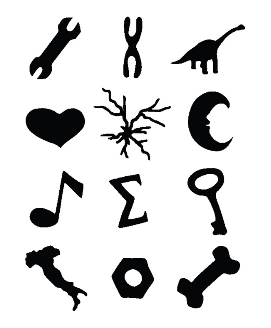
\includegraphics[width=.35\linewidth]{./img/shapes.png}
    \legend{Fonte: \citeonline{book_shape}. }
    \label{fig:shape}
\end{figure}

Curvas na dimensão $\mathbb{R}^2$ são definidas por funções $F: A \rightarrow \mathbb{R}^2$, com $F$ de classe $C^2$ e $A \subseteq \mathbb{R}$ intervalo fechado - ou seja, funções de uma variável real a valores em $\mathbb{R}^2$. Nestas, cada valor t $\in$ $A$ é associado a um vetor bidimensional. Em imagens, podem ser visualizadas curvas em contornos de figuras.

A partir de uma amostragem finita de pontos pode-se reconstruir curvas e superfícies. Existem diversos algoritmos com tal finalidade, podendo ser baseados majoritariamente em técnicas interpolatórias, funções implícitas ou geração de malhas \cite{book_sorkine}.

Os baseados em técnicas interpolatórias normalmente se baseiam na triangulação de Delaunay \cite{compgeometry} e respectiva interpolação dos pontos e, por isso, tem custo computacional alto. Já as técnicas baseadas em funções implícitas realizam a representação das curvas e superfícies por um conjunto de funções implícitas e, portanto, permitem a realização de operações padrões matemáticas com estas funções, porém impossibilitam o percurso sobre a superfície - porém, são mais adequadas que técnicas interpolatórias se a nuvem de pontos tiver ruídos. Os métodos baseados em malhas realizam a reconstrução de superfícies a partir de uma quantidade definida de malhas (quanto mais malhas, mais próxima a superfície reconstruída fica da original). Em casos bidimensionais, não são consideradas malhas, mas sim curvas poligonais.

A extração de características robustas a partir de imagens, proposta neste projeto de Iniciação Científica, é parte de uma das linhas do projeto temático (FAPESP $2019/07316-0$), intitulado \textit{Teoria de singularidades e aplicações a geometria diferencial, equações diferenciais e visão computacional}. Das 4 linhas de atuação do projeto, uma diz respeito à reconstrução de faces humanas a partir de informações reduzidas do domínio. Por exemplo, deseja-se reconstruir uma face humana (nariz, boca, olhos dentre outros elementos) a partir de uma versão simplificada desta (por exemplo, uma caricatura representada por curvas simplificadas da face). O ponto de partida para esta reconstrução é a identificação das características robustas.      

% ----------------------------------------------------------
% Objetivos
% ----------------------------------------------------------
\chapter{Objetivos}

O objetivo principal deste projeto de pesquisa é extrair características robustas em $\mathbb{R}^2$ para reconstrução de curvas com alta precisão a partir de imagens. 

A realização desta tarefa implica na observância dos seguintes objetivos específicos:

\begin{itemize}
    \item Pré-processar as imagens visando a eliminação de ruídos,  binarização e consequente segmentação;
    \item Extrair atributos de formas das imagens (contorno e cálculo da curvatura);
    \item Determinar as características robustas por análise da curvatura;
    \item Reconstruir as formas a partir das características robustas, por meio de curvas poligonais e operadores Laplacianos como sugerido por \citeonline{book_sorkine} e 
    \item Aferir a qualidade da reconstrução a partir da curva original.
\end{itemize}

%Assim sendo, a presente pesquisa visa desenvolver e analisar algoritmos eficientes para o pré-processamento de imagens, extração de contorno de objetos da imagem, extração dos pontos importantes da curva deste contorno, e a respectiva reconstrução de curvas a partir desses pontos, processos estes que terão suma importância para o mapeamento de características robustas entre espaços $\mathbb{R}^2$ e $\mathbb{R}^3$.

% \chapter{Objetivo geral}

%  \begin{itemize}
%   \item Organizar algoritmos sobre a extração de pontos importantes de curvas discretas e a reconstrução de curvas a partir destes.
%  \end{itemize}

% \chapter{Objetivos específicos}

%  \begin{itemize}
%   %\item Examinar algoritmos populares em processamento de imagens.
%   \item Binarizar imagens por meio de técnicas de pré-processamento.
%   \item Extrair contornos em imagens.
%   \item Calcular curvaturas de contornos.
%   \item Localizar pontos importantes em curvas discretas.
%   \item Desenvolver códigos eficientes para reconstrução de curvas discretas a partir de pontos de controle.
%   %\item Pesquisar aplicações de mapeamentos de características robustas bidimensionais em tridimensionais.
%  \end{itemize}
 
% ----------------------------------------------------------
% Fundamentos
% ----------------------------------------------------------
\chapter{Conceitos básicos e fundamentos teóricos}

A execução deste projeto requer o conhecimento em áreas de conhecimentos distintos, que vão do processamento de imagens à geometria diferencial.  Nesta seção, serão detalhados os principais conceitos necessários ao desenvolvimento do trabalho.

\section{Pré-processamento em imagens}

Para se extrair contornos em imagens reais, muitas vezes é necessário realizar operações de pré-processamento.  Tais processos são de naturezas diversas, envolvendo desde a conversão de modelos de cores à segmentação. As principais atividades são descritas a seguir. 

\subsection{Suavização}

A partir de imagem em escalas de cinza, realiza-se a suavização da imagem, com o objetivo de eliminar ruídos. O método mais simples de suavização é a aplicação de filtro gaussiano \cite{szeliski}.

O filtro gaussiano pode ser realizado a partir da seguinte equação:

$$G(x) = \frac{1}{2\pi\sigma^2}e^{-\frac{x^2}{2\sigma^2}},$$ em que $\sigma$ representa o desvio padrão, com média 0 (ou seja, é uma distribuição gaussiana centrada na origem). Esta distribuição é então utilizada como uma função para propagar os pontos da imagem a partir de uma convolução. Quanto maior o valor de $\sigma$, maior o efeito de borramento produzido na imagem.

Porém, o filtro gaussiano possui a propriedade de borrar a imagem de forma indistinta, tanto em regiões de baixa como de alta frequência. Isso pode provocar, por exemplo, o deslocamento de bordas que definem contornos importantes dos objetos. Neste projeto, é importante extrair contornos precisos, que sejam fiéis ao real contorno dos objetos presentes na imagem.

Para situações que requerem a preservação de bordas e ao mesmo tempo suavização em regiões de baixa frequência, é possível aplicar o filtro de difusão anisotrópica Perona Malik \cite{perona_malik}. Seja $\Omega \subset \mathbb{R}^2$ e $I(x, y, t)$ em $\Omega$ a imagem suavizada no tempo $t$ (sendo a imagem original quando $t = 0$). A difusão anisotrópica é definida como:

$$\frac{\partial I}{\partial t} = div(c(x, y, t) \nabla (I(x, y, t))) = \nabla (c(x, y, t)) \cdot \nabla (I(x, y, t))) + c(x, y, t) \nabla (I(x, y, t))),$$ sendo $\nabla$ o gradiente, $div(...)$ o operador divergência e escolhendo o coeficiente de difusão $c(x, y, t) = g(|\nabla I(x, y)|)$. Com isso, \citeonline{perona} propuseram duas funções para a função de difusão $g(|\nabla I(x, y)|)$:

\[ 
g_1(|\nabla I(x, y)|) = exp \left \{  -\left[ \frac{|\nabla I(x, y)|}{k} \right]^2 \right \}
\]
\[
g_2(|\nabla I(x, y)|) = \frac{1}{1 + \left( \frac{|\nabla I(x, y)|}{k}  \right)^2}
\]

Tais funções, em regiões de alta frequência, identificadas pela computação do gradiente, fazem com que o filtro reduza o seu efeito de filtragem. Na prática, produz uma imagem em que as bordas são preservadas em suas posições originais, ao mesmo tempo que suaviza áreas de baixa frequência. 

\subsection{Binarização}

Uma maneira eficiente para se obter o contorno de um objeto é transformar a imagem em uma presentação binária. Uma imagem binária possui pixels de valores 0 ou 1, em que 1 representa posições do plano superior e 0 representa o plano de fundo \cite{burger}.

A binarização pressupõe a existência de um parâmetro conhecido como limiar. Todo pixel com valor maior ou igual terá valor binário 1, enquanto os de valor menor terão valor binário 0.

A questão mais importante deste processo é a escolha automática do limiar. Para isso, pode-se utilizar o método de Otsu \cite{otsu_method}. O algoritmo de Otsu calcula o valor de um limiar $t$ que minimiza a variância ponderada intra-classes, dada pela relação: 
\[
\sigma_w^2(t) = q_1(t)\sigma_1^2(t)+q_2(t)\sigma_2^2(t)
\]

\noindent sendo as probabilidades de cada classe (objeto e fundo, por exemplo) estimadas por:

\[
q_1(t) = \sum_{i=1}^{t} P(i) \quad \& \quad q_2(t) = \sum_{i=t+1}^{I} P(i)
\]

\noindent e as médias de ambas as classes computadas como:

\[
\mu_1(t) = \sum_{i=1}^{t} \frac{iP(i)}{q_1(t)} \quad \& \quad \mu_2(t) = \sum_{i=t+1}^{I} \frac{iP(i)}{q_2(t)}
\]

Finalmente, as variâncias para cada classe podem ser assim calculadas: 

\[
\sigma_1^2(t) = \sum_{i=1}^{t} [i-\mu_1(t)]^2 \frac{P(i)}{q_1(t)} \quad \& \quad \sigma_2^2(t) = \sum_{i=t+1}^{I} [i-\mu_2(t)]^2 \frac{P(i)}{q_2(t)}
\]

Para uma imagem em nível de cinza, basta percorrer a faixa de valores $t=0,\dots,255$ e escolher aquele que minimiza  $\sigma_w^2(t)$.

\subsection{Erosão e dilatação}

Outro ponto importante da pré-segmentação diz respeito a operadores elementares da morfologia matemática \cite{serra} - a erosão e a dilatação.

De acordo com \citeonline{jserra}, a dilatação é feita com o objetivo de preencher pequenos buracos e ampliar a figura original, de modo a eliminar pequenas imperfeições formadas por outros pré-processamentos aplicados ou pela falta de informações na imagem original. Formalmente, sendo $A$ um conjunto de pixels, $B$ um elemento estruturante e $z$ os valores de primeiro plano, a operação de dilatação $A \oplus B$ é definida como:

\[
A \oplus B = \{z | (\hat{B})_z \cap A \neq \emptyset\}
\]

Já a erosão é feita com o objetivo de ``diminuir'' o objeto, podendo expandir ``buracos'', remover pequenas áreas e separar regiões próximas. Formalmente, a operação de erosão $A \ominus B$ entre o conjunto $A$ e o elemento estruturante $B$ é definida como:

\[
A \ominus B = \{z | (B)_z \subseteq A\}
\]

%\todo[inline]{FAlta uma referencia aqui também.... O cara que "inventou" a morfologia matemática para Proc Imagems foi Jean Serra... veja a referencia... Mathematical Morphology and Its Applications to Image Processing, J. Serra and P. Soille (Eds.), proceedings of the 2nd international symposium on mathematical morphology (ISMM'94), ISBN 0-7923-3093-5 (1994) Pode também citar o livro do Gonzalez....}

\subsection{Extração de contorno}

A partir da imagem pré-processada, o contorno de um objeto binário pode ser obtido por métodos de extração de contornos. Uma maneira importante de representar um contorno é de forma parametrizada, análoga à representação de curvas em geometria diferencial \cite{szeliski}.

Um algoritmo utilizado para esta extração, definido em \citeonline{book_shape}, é o algoritmo de \textit{contour following}, que acompanha a borda do objeto a partir de um ponto inicial, analisando se os pontos vizinhos também pertencem ao objeto em questão. Os passos inicial (a) e final (b) deste algoritmo podem ser visualizados na figura \ref{fig:contorno}.

Este método tem como entrada uma imagem binária e, como saída, um vetor de coordenadas, que representa o contorno externo do objeto.

\begin{figure}[htb]
\centering
    \caption{Representação do algoritmo de extração de contorno}
    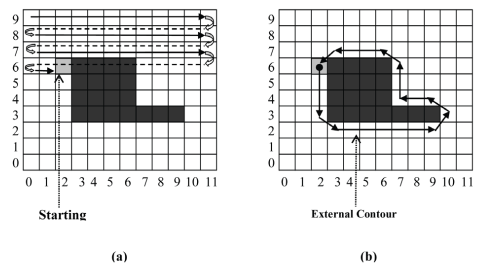
\includegraphics[width=.7\linewidth]{./img/contorno.png}
    \legend{Fonte: \citeonline{book_shape}. }
    \label{fig:contorno}
\end{figure}

\section{Cálculo de curvatura}

De acordo com \citeonline{book_curvatura}, curvatura é a taxa de mudança na direção da aresta, em que as curvas estão presentes nos contornos (definidos por arestas).

A curvatura de uma curva regular parametrizada por uma aplicação $t \rightarrow (x(t), y(t))$, onde $x(t)$ e $y(t)$ são funções de classe $C^2$, é dada por:

$$\kappa (t) = \frac{x'(t) y''(t) - y'(t) x''(t)}{(x'(t)^2 + y'(t)^2)^{3/2}}$$

Porém, caso a curva seja extraída diretamente da imagem, usamos a curvatura discreta da curva, obtida como descrito a seguir. A partir de detecção de contornos, pode-se utilizar operações vetoriais, como a diferença da direção de arestas entre pixels vizinhos da curva do modo

$$\kappa (t) = \varphi_{t+1} - \varphi_{t-1},$$ em que $\varphi_t$ é a direção do gradiente do pixel $t$ da curva. Alternativamente, pode-se calcular a direção do gradiente do pixel diretamente pela posição dos pixels:

$$\kappa (t) = \frac{y_{t - 1} - y_{t+1}}{x_{t - 1} - x_{t+1}}$$

\section{Características robustas}

A menos de translação e rotação, uma curva pode ser determinada por sua curvatura. Considerando o gráfico da curva, os pontos de destaque são as intersecções com o eixo-x e os pontos de máximos e mínimos (locais e globais) - ver figura \ref{fig:caractrobust}.

Os pontos de intersecção com o eixo-x representam os pontos de inflexão da curva, e os pontos extremos representam os vértices da curva. Tais pontos são denominados características robustas da curva. Observe que, pelo teorema dos quatro vértices \cite{book_manfredo}, toda curva fechada e simples tem, pelo menos, quatro vértices.

\begin{figure}[htb]
\centering
    \caption{Demarcação dos pontos importantes de uma curva com $\kappa(x) = x^3 - 2x$}
    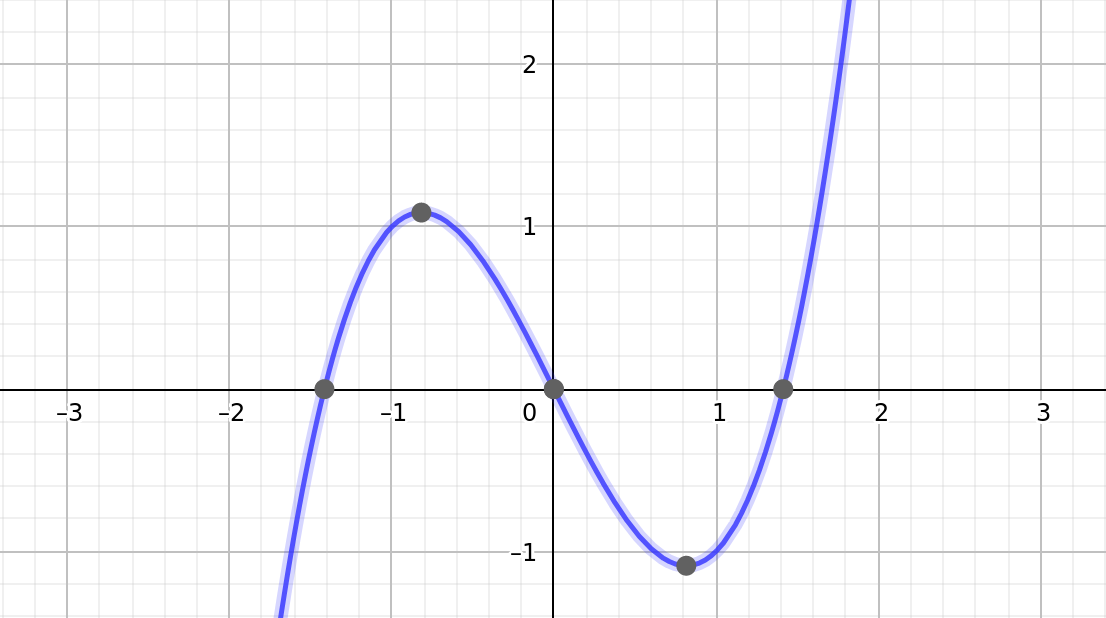
\includegraphics[width=.5\linewidth]{./img/curva.png}
    \legend{Fonte: Elaborada pelo autor. }
    \label{fig:caractrobust}
\end{figure}

As características robustas podem ser determinadas em curvas a partir de cálculos de curvatura e da sua derivada.

\section{Reconstrução de curvas}

A reconstrução de curvas a partir de imagens ou pontos de controle é de fundamental importância em áreas como computação gráfica, geometria computacional, visão computacional e processamento de imagens. Boa parte de soluções neste campo baseiam-se em representações do tipo \emph{spline} \cite{Schoenberg1946}. Técnicas baseadas em \emph{spline} consistem basicamente de um processo de minimização da distância entre a curva de referência e o resultado obtido e são ditas interpolatórias, uma vez que a curva resultante passa por todos os pontos de controle. \citeonline{Jakbczak2014} mostra como interpolar uma curva 2D a partir de um conjunto de pontos usando informação sobre a distribuição probabilística dos pontos faltantes. Mais recentemente \cite{DeepSpline} o uso de aprendizado profundo foi explorado juntamente com splines para a reconstrução de curvas paramétricas e superfícies. 

Uma segunda categoria de reconstrução de curvas são as baseadas em aproximação em que não necessariamente a curva ou superfície é reconstruída passando pelos pontos de controle. \citeonline{Lee2000} propõe um método baseado em mínimos quadrados combinado à uma árvore geradora mínima Euclidiana para, a partir de um conjunto de pontos não organizados, aproximar uma curva. 


Uma forma alternativa para reconstruir curvas a partir de um conjunto de pontos é descrita por \citeonline{book_sorkine}. A abordagem é baseada no operador de Laplace e representações diferenciais entre os vértices de uma dada vizinhança em uma malha de pontos. Em contraste com tradicional representação por coordenadas cartesianas globais, a representação diferencial de uma superfície revela informações sobre a forma local da mesma, bem como o tamanho e orientação de detalhes locais. Além de prover informações que resultarão em uma reconstrução com maior preservação de detalhes, trata-se de um sistema linear o que o torna computacionalmente eficiente.

\subsection{O Operador Laplaciano e a representação diferencial}


Seja uma malha triangular caracterizada por $M = (V,E,F)$, contendo $V$ vértices, $E$ arestas e $F$ faces. Cada vértice $i$ de $M$ possui uma representação cartesiana dada por $\mathbf{v}_i = (x_i,y_i,z_i)$. Coordenadas diferenciais (também conhecidas como $\delta-coordenadas$) de $\mathbf{v}_i$ são definidas como a diferença entre a coordenada Cartesiana e o centro de massa de seus vizinhos imediatos na malha:

\begin{equation}
    \delta_i = (\delta_i^x, \delta_i^y, \delta_i^z) = \mathbf{v}_i - \frac{1}{d_i} \sum_{j \in N(i)} \mathbf{v}_j,
    \label{eq_delta}
\end{equation}

\noindent onde $N(i) = \{j|(i,j) \in E$ e $d_i = |N(i)|$ é o número dos vizinhos imediatos de $i$. 

Como ilustra a figura \ref{fig:coordDif}, as coordenadas diferenciais aproxima não apenas as características da forma local da superfície, mas também a direção normal e a curvatura média. 

\begin{figure}[htb]
\centering
    \caption{O vetor da coordenada diferencial em um vértice aproxima a forma local superfície: representação da direção normal e da curvatura média}
    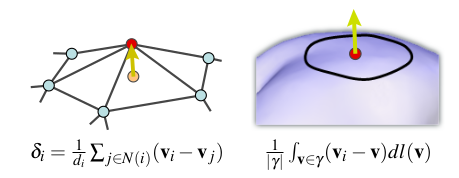
\includegraphics[width=.5\linewidth]{./img/difcoord.png}
    \legend{Fonte: \citeonline{book_sorkine}. }
    \label{fig:coordDif}
\end{figure}


A equação \ref{eq_delta} pode ser também representada em forma matricial, o que simplifica os cálculos. Seja a matriz de adjacência como definida pela equação \ref{eq_matadj}  e a matriz diagonal $D$, com $D_{ii} = d_i$:

\begin{equation}
    A_{i,j} = \begin{cases}
        1, & (i,j) \in E\\
        0, & \text{caso contrário}.
        \end{cases}
     \label{eq_matadj}
\end{equation}

A matriz Laplaciana pode então ser calculada pela equação \ref{eq_laplaciana} ou \ref{eq_laplacianaSimet}, que é uma versão simétrica. A figura \ref{fig:matrizLaplaciana} ilustra um exemplo de uma simples malha triangular e sua respectiva representação matricial Laplaciana.

\begin{equation}
    L_s = D-A
    \label{eq_laplaciana}
\end{equation}

\noindent ou mesmo

\begin{equation}
    (L_s)_{ij} = \begin{cases}
        d_i, & (i = j)\\
        -1, & (i,j) \in E \\
         0, & \text{caso contrário}.
        \end{cases}
     \label{eq_laplacianaSimet}
\end{equation}

\begin{figure}[htb]
\centering
    \caption{Uma malha triangular e sua respectiva matriz Laplaciana $L_s$}
    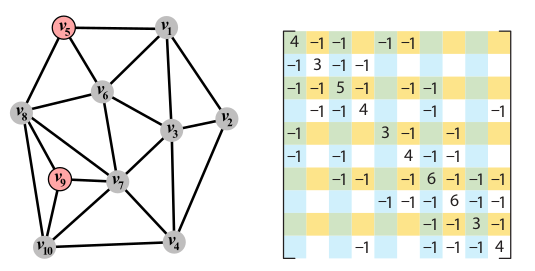
\includegraphics[width=.5\linewidth]{./img/meshLaplacian.png}
    \legend{Fonte: \citeonline{book_sorkine}. }
    \label{fig:matrizLaplaciana}
\end{figure}


Uma melhor aproximação para as coordenadas diferenciais foi empregada por \cite{Pinkall1993} ao considerar pesos não uniformes para os vértices vizinhos. 


\subsection{Reconstrução de curvas a partir das \texorpdfstring{$\delta$} --coordenadas}

A princípio, dado \textbf{um conjunto} de $\delta-coordenadas$, não é possível restaurar as coordenadas globais originais, pois a matriz $L_s$ é singular, ou seja, a expressão $\mathbf{x} = L^{-1} \delta^{(x)}$ é indefinida. 

No entanto, existe solução para este problema, por meio da resolução de um sistema linear do tipo \textbf{full-rank} dado por 


\begin{equation}
    \Tilde{\mathbf{x}} = \argmin_\mathbf{x} \left( ||L\mathbf{x} - \delta^{(x)}||^2 + \sum_{j \in C} \omega^2 |x_j - c_j|^2 \right)
    \label{eq_LeastSquare_linearSyst}
\end{equation}

\noindent onde $\mathbf{x}$ é um vetor de dimensão n que contém as coordenadas absolutas $x$ de todos os vértices; $C$ é o conjunto dos índices dos vértices cuja localização espacial é conhecida - o conjunto de vértices em $C$ são restrições impostas ao sistema - também conhecidas como âncoras e $\omega > 0$ é o peso que regula a importância atribuída a posição de cada restrição. \citeonline{book_sorkine} detalha um método eficiente para se resolver o problema de mínimos quadrados da equação \ref{eq_LeastSquare_linearSyst}. 

A matriz $L_s$ possui propriedades espectrais que são fundamentais para a reconstrução de curvas a partir de um conjunto de pontos. Por ser simétrica  semi-definida positiva, esta possui uma base de autovetores ortogonal $E = \{ \mathbf{e}_1, \mathbf{e}_2, \ldots, \mathbf{e}_n \}$. Sejam os autovalores representados por $\lambda_i$, $0 = \lambda_1 < \lambda_2 \leq \lambda_3 \leq \ldots \leq \lambda_n$. Sabe-se que os menores autovalores não zero $\lambda_i$ são muito pequenos e o maior autovalor $\lambda_n$ está associado ao vértice de maior valência na malha $M$. Os primeiros autovetores (associados aos menores autovalores) são suaves, enquanto os maiores têm mais altas frequências. A base Laplaciana de autovalores e autovetores é, de fato, uma extensão da base discreta de cosseno para domínios irregulares \cite{Taubin1995}. Portanto, pode-se dizer que autovalores são considerados frequências de uma malha. 

Encontrar uma boa base para a representação compacta de uma forma, ou curva, significa que é possível usar somente uma fração de tal base para se aproximar de forma apropriada uma determinada geometria. Em processamento de imagens, por exemplo, pode-se utilizar bases de wavelet ou Fourier. A figura \ref{fig:reconstrucao} ilustra um exemplo de reconstrução por meio de duas bases: a base de autovetores Laplaciana e uma base sensível à geometria \cite{Sorkine2005}. Repare que segunda base provê uma melhor aproximação, tanto em maior quanto em menor escala.


%De acordo com \citeonline{book_sorkine}, existem diversos algoritmos para reconstrução de curvas e superfícies a partir de pontos finitos. Uma maneira de realizar esta reconstrução é a partir de representação de curvas lineares por partes, que provê informações sobre a visualização da curva e suas características topológicas. Esta representação pode necessitar de processamento geométrico (como filtragem, re-amostragem e compressão), visto que os pontos de entrada podem conter ruídos ou informações desnecessárias.

%Este método pode ser realizado a partir de operadores de Laplace discretos, calculando-se a matriz de Laplace referente aos pontos originais \cite{book_sorkine}.

%\todo[inline]{Acho que poderia ter uma referência sobre operadores discretos de Laplace..... }

%Na figura \ref{fig:reconstrucao} pode-se observar um exemplo de reconstrução de uma curva a partir de finitos pontos.

%\begin{figure}[htb]
%\centering
%    \caption{Reconstrução de uma curva fechada}
%   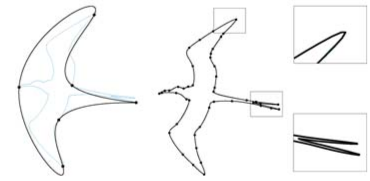
\includegraphics[width=.5\linewidth]{./img/reconstrucao.png}
%    \legend{Fonte: \citeonline{book_sorkine}. }
%    \label{fig:reconstrucao}
%end{figure}

\begin{figure}[ht]
\caption{Reconstrução de uma curva fechada usando bases distintas. A reconstrução é é representada pela curva negra e a curva original pelo traçado em azul. As âncoras são representadas pelos pontos negros: a) base autovetores Laplaciana 6 e 45 vértices, respectivamente; b) base sensível à geometria, também com 6 e 45  vértices, respectivamente}
\begin{subfigure}{.47\textwidth}
  \centering
  % include first image
  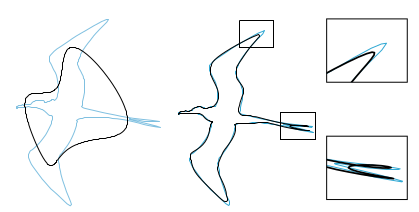
\includegraphics[width=.8\linewidth]{./img/reconstrucao1.png}  
  \caption{Base autovetores Laplacianos}
\end{subfigure}
\begin{subfigure}{.5\textwidth}
  \centering
  % include second image
  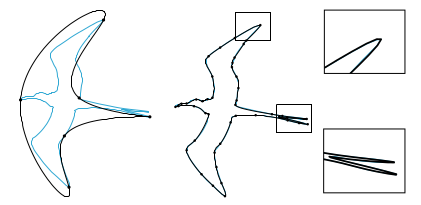
\includegraphics[width=.8\linewidth]{./img/reconstrucao2.png}  
  \caption{Base sensível à geometria}
\end{subfigure}

\legend{Fonte: \citeonline{book_sorkine}.}
\label{fig:reconstrucao}
\end{figure}


\section{Métricas para avaliação de similaridades entre contornos}
\label{sec:evaluation}

A similaridade entre curvas paramétricas, cuja representação consiste apenas de um vetor de pontos, pode ser computada simplesmente por meio de métodos tradicionais de distância entre cada par de pontos (tanto da curva de referência quanto da curva reconstruída), como por exemplo a Distância Euclidiana ou Distância de Manhattan. No entanto, há diversas outras métricas que podem ser usadas para avaliar quantitativamente a similaridade entre dois contornos, largamente utilizadas em aplicações de visão computacional e processamento de imagens. A seguir, serão apresentadas 3 métricas: uma baseada na cobertura de regiões; a segunda, na distância entre os contornos de objetos e a terceira, uma medida baseada em probabilidades.  

\subsection{Covering} Seja  $S_T$ o resultado da segmentação e $S_G$ uma segmentação de referência (padrão outro). A cobertura de regiões (\textit{covering}) \cite{Crevier} quantifica a cobertura das regiões de $S_T$ em relação às regiões de $S_G$. Esta é definida por: 
\begin{equation}
  \label{eq:imagesegmetric1}
    \begin{split}
    {Covering(S_T\to S_G)} &= {\frac{1}{A}\sum_{R \in S_G}{|R|\ \underset{R' \in S_T}{\operatorname{max\ }} {\{ \mathcal{O}(R,R')} \}} },
    \end{split}
  \end{equation}

  \begin{equation}
  \label{eq:towregions}
    \begin{split}
    {\mathcal{O}(R,R')} &= {\frac{|R \cap R'|}{|R \cup R'|}} = {\frac{|R \cap R'|}{|R|+|R'| - |R \cap R'|}},
    \end{split}
  \end{equation}
  
\noindent onde  $A$ é o número de pixels na imagem;  $R$ e $R'$ são as regiões de $S_G$ e $S_T$, respectivamente;
$\mathcal{O}(R,R')$ representa a sobreposição entre as regiões de  $R$ e $R'$ e $|R|$ e $|R'|$ o número de pixels nas regiões de $R$ e $R'$, respectivamente. Eq. \ref{eq:imagesegmetric1} retorna valores na faixa $(0,1)$. Quanto maior o valor, maior a similaridade entre $S_T$ e $S_G$. Esta métrica pode ser usada no contexto deste projeto, em especial em casos de curvas fechadas.

\subsection{Medida Baseada em contornos} 
\label{sc:boundarybm}
A avaliação de similaridade por contornos \cite{HuangDom} pode ser quantificada ao calcular-se a distância mínima entre pares de pontos de 2 conjuntos distintos: (i) $BT$, os contornos produzidos por um método de segmentação $S_T$ e (ii) $BG$, os contornos de um padrão ouro $S_G$. A similaridade resultante vem do cálculo das medidas de Precisão (P), Revocação (R) e de BF1-Score, dadas por:

\begin{equation}\label{eq:p:metric}
P = 
\frac{1}{|BT|} \sum_{p \in BT }^{}[Matched(p,BG) \leq \theta]
\end{equation}
\begin{equation}\label{eq:r:metric}
R = 
\frac{1}{|BG|}\sum_{p \in BG}^{}[Matched(p,BT) \leq \theta]
\end{equation}
\begin{equation}\label{eq:f:metric}
 	\begin{split}
		BF1-Score &= 2 \times{\frac{P \times R}{ R+P}},
		%F1 Score &= \frac{PR}{\alpha R+(1-\alpha P)},
    \end{split}
\end{equation}

A função  $Matched(.)$, em $P$, percorre os pontos $p$ de BT em busca dos pontos mais próximos dos contornos em $BG$, de acordo com a distância máxima $\theta$. Se $[.]$ for verdade, esta retorna $1$, caso contrário, $0$. A função $Matched(.)$, em $R$, percorre os pontos $p$ de $BG$ em busca dos pontos próximos aos contornos de $BT$. $|BT|$ e $|BG|$ são os números de pontos existentes em BT e BG, respectivamente.

\subsection{Probabilistic Rand Index (PRI)}
A métrica PRI \cite{Unnikrishnan} computa a probabilidade de um par de pixels $(i,j)$ pertencer aos contornos resultantes de um método de segmentação $S_{T}$, contendo rótulos consistentes em um conjunto $k$ de um método de segmentação de referância $S_{G_{k}}$ (padrão ouro). A métrica PRI é definida por:
\begin{equation}
    \label{eq:pri}
    PRI(S_{T}, \{S_{G_k}\})=\frac{1}{A}\sum_{i<j}^{}\left[c_{ij}p_{ij}+(1-c_{ij})(1-p_{ij})\right]
\end{equation}

\noindent onde $c_{ij}$ é a probabilidade dos pixels $i$ e $j$ possuírem o mesmo rótulo na segmentação $S_T$ e $p_{ij}$ corresponde à probabilidade dos pixels $i$ e $j$ compartilharem os mesmos rótulos na segmantação de referência $S_{G_{k}}$, e $A$ é o total do número de pares de pixels. A função PRI retorna valores na faixa $(0,1)$. Quanto maior o valor, maior a similaridade entre $S_{T}$ e $S_{G_{k}}$.


% Existem vários algoritmos para a reconstrução de curvas a partir de finitos pontos. Por exemplo, podem ser utilizados métodos baseados em técnicas interpolatórias, funções implícitas ou geração de malhas \cite{book_sorkine}.

% Em espaços bidimensionais, objetiva-se fazer.

% Os métodos baseados em técnicas interpolatórias, como o nome sugere, realizam a interpolação de pontos vizinhos para a reconstrução. Neste processo, é comumente utilizada a triangulação de Delaunay, algoritmo computacionalmente custoso.

% As técnicas baseadas em funções implícitas representam as curvas das figuras como um conjunto de funções implícitas, calculadas a partir de alguma função de base radial. Esta forma de representação permite ainda a utilização de operações \textit{booleanas}, possibilitando, por exemplo, a intersecção da figura com outros objetos.

% Um outro método para reconstrução de curvas é realizado a partir de geração de malhas. Pode-se também realizar tratamentos e processamentos nas malhas geradas, de modo a, por exemplo, deixar as curvas de determinada figura mais "suave".

% ----------------------------------------------------------
% Material e métodos
% ----------------------------------------------------------
\chapter{Materiais e métodos}

O diagrama de blocos da Figura \ref{fig:diagrama} ilustra as principais etapas de desenvolvimento deste projeto de pesquisa. 

\begin{figure}[htb]
\centering
    \caption{Diagrama de bloco das etapas de desenvolvimento}
    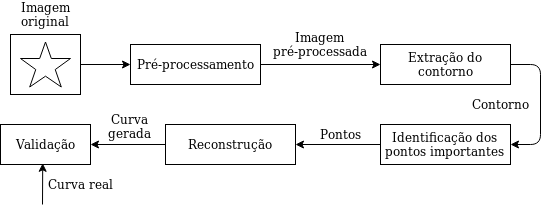
\includegraphics[width=.7\linewidth]{./img/diagrama.png}
    \legend{Fonte: Elaborada pelo autor.}
    \label{fig:diagrama}
\end{figure}

Neste projeto, optou-se inicialmente por empregar um banco de dados de folhas do \textit{ImageCLEF 2011} (Figura \ref{fig:folha}). Seu uso se justifica pela necessidade de avaliarmos o método com precisão. Ao observarmos tais imagens é possível perceber que os contornos podem ser extraídos com uma certa facilidade e com alta precisão. Estes contornos serão utilizados como padrão ouro no processo de validação do método.

\begin{figure}[htb]
\centering
    \caption{Exemplo de folhas do banco de dados utilizado}
    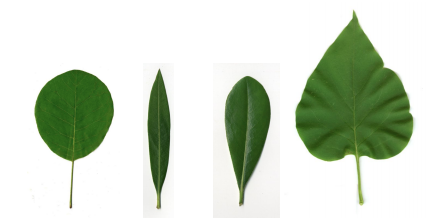
\includegraphics[width=.5\linewidth]{./img/folhas.png}
    \legend{Fonte: \citeonline{imageclef_2011}. }
    \label{fig:folha}
\end{figure}

O pré-processamento consistirá em simplificar as imagens a partir de métodos de binarização, segmentação e remoção de ruídos, de modo a deixá-las preparadas para as etapas seguintes. A morfologia matemática poderá, se necessário, ser empregada na imagem binária para eliminar pequenos ``buracos'' no interior da imagem ou pontos espúrios ao longo da borda.

Será então obtido o contorno da imagem pré-processada, que será representado como curvas discretas. Nestas serão feitas cálculos de variação de curvatura, de modo a encontrar seus pontos importantes.

A partir dos pontos importantes (ou características robustas) será feita a reconstrução das curvas.

%Serão utilizadas, como métricas para verificação de erros, a distância entre os pontos das curvas geradas e das curvas originais, ambas calculadas a partir das imagens de entrada originais.

Com as curvas originais extraídas das imagens e as curvas geradas pelo algoritmo de reconstrução a partir de pontos importantes, os resultados podem ser avaliados por meio de métodos tradicionais de distância entre pontos (entre os pontos corretos das curvas e os pontos gerados pelo algoritmo) ou por meio das métricas descritas na seção \ref{sec:evaluation}.

Vale lembrar que esta proposta é parte de um projeto temático que visa a reconstrução de elementos de uma face humana. Propomos também avaliar os métodos implementados com base em dados reais de faces e caricaturas humanas (como exemplo na figura \ref{fig:stallone}). A diferença é que neste tipo de imagem teremos não apenas um contorno, mas uma coleção destes.  

\begin{figure}[htb]
\centering
    \caption{Caricatura humana}
    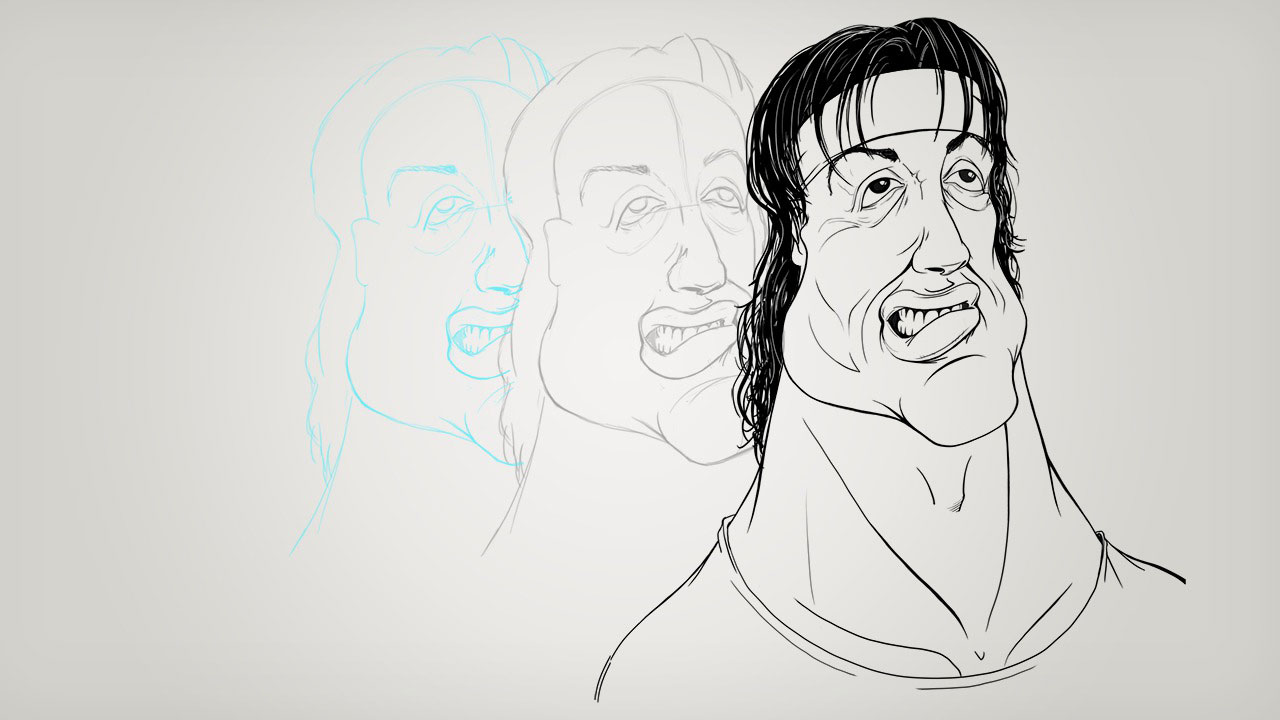
\includegraphics[width=.5\linewidth]{./img/Stalon.jpg}
    \legend{Fonte: \citeonline{stallone}. }
    \label{fig:stallone}
\end{figure}

O projeto será implementado em plataforma Linux, com as linguagens de programação \textit{MatLab} e, caso necessário, \textit{Python}, utilizando-se bibliotecas padrões destas linguagens. Também poderá ser utilizada a linguagem \textit{C++}, caso seja necessária uma implementação com menor tempo de execução.

%\todo[inline]{O conteúdo da seção 5 já tinha sido colocado na metodologia.. Eu achei melhor retirá-lo. Transferi o conteúdo dele para a metodologia...}

% ----------------------------------------------------------
% Forma de análise dos resultados
% ----------------------------------------------------------
%\chapter{Forma de análise dos resultados}
%Com as curvas originais extraídas das imagens e as curvas geradas pelo algoritmo de reconstrução a partir de pontos importantes, os resultados podem ser analisados a partir de métodos tradicionais de distância entre pontos (entre os pontos corretos das curvas e os pontos gerados pelo algoritmo), como a \textit{Distância Euleriana} e a \textit{Distância de Manhattan}.

% ----------------------------------------------------------
% Plano de trabalho e cronograma
% ----------------------------------------------------------

\chapter{Plano de trabalho e cronograma}

%Primeiramente no desenvolvimento da pesquisa será realizado o estudo em pré-processamento das imagens, com o objetivo de prepará-las para as fases posteriores do projeto. Após isso, serão feitas pesquisas específicas sobre métodos de extração de contornos em imagens, e a respectiva codificação destes métodos.

%Com os pontos já extraídos, terá início a pesquisa sobre extração de pontos importantes nas curvas e algoritmos eficientes.  A partir deles terá início a pesquisa sobre métodos e algoritmos eficientes sobre reconstruções de curvas. Com os resultados obtidos serão feitas avaliações e testes. 

As ações definidas neste projeto de iniciação científica serão executadas de acordo com o cronograma definido na tabela \ref{tab:cronograma}. Como o aluno já tem noções de processamento de imagens, acreditamos que as etapas de pré-processamento e extração de contornos será feita em menor tempo. A etapa que demandará mais esforço, que inclui não apenas a implementação mas o estudo e compreensão do método de \citeonline{book_sorkine}, será a reconstrução da curva a partir dos pontos importantes.

Durante todo o andamento do projeto serão realizadas reuniões periódicas com professores - tanto o orientador quanto outros professores da equipe do projeto temático - de modo a complementar e auxiliar a pesquisa. Vale ressaltar que o candidato tem participado regularmente de tais reuniões (atualmente em modo sempre virtual) que acontecem semanalmente.


\begin{table}[htb]
\footnotesize
\centering
\vspace{0.5em}
\setlength{\tabcolsep}{0.05in}
\begin{tabular}{|c|c|c|c|c|c|c|}
\hline
Atividades
& \multicolumn{6}{c|}{Meses de trabalho} \\
\cline{2-7}
& 1\textordmasculine\ e 2\textordmasculine & 3\textordmasculine\  e 4\textordmasculine & 5\textordmasculine\  e 6\textordmasculine & 7\textordmasculine\  e 8\textordmasculine & 9\textordmasculine\  e 10\textordmasculine & 11\textordmasculine\  e 12\textordmasculine \\ \hline
 %Familizariação com processamento de imagens & $\bullet$ & & & & &\\ \hline
 Estudo das técnicas de reconstrução de curvas  & $\bullet$ & $\bullet$ & & & &\\ \hline
 Pré-processamento e Extração de contornos & & $\bullet$ & $\bullet$ & & & \\ \hline
 Extração dos pontos importantes & & $\bullet$ & $\bullet$ & & & \\ \hline
 Redação do relatório parcial & & & $\bullet$ & & & \\ \hline
 Implementação da reconstrução de curvas & & & & & & \\
 (Sorkine)& & & $\bullet$ & $\bullet$ & $\bullet$ & \\ \hline
 Avaliação e testes & & & & $\bullet$ & $\bullet$ & \\ \hline
 Desenvolvimento do relatório final & & & & & $\bullet$ & $\bullet$ \\ \hline
\end{tabular}
\caption{Cronograma de atividades para 12 meses de trabalho.}
\label{tab:cronograma}
\end{table}

\nocite{book_bruce}

\endgroup

% ----------------------------------------------------------
% ELEMENTOS PÓS-TEXTUAIS
% ----------------------------------------------------------
\postextual

% ----------------------------------------------------------
% Referências bibliográficas
% ----------------------------------------------------------
\bibliography{referencias}

%---------------------------------------------------------------------
% INDICE REMISSIVO
%---------------------------------------------------------------------
\phantompart

\printindex

\end{document}